\section{Defining a Community Core}

Previous attempts for identifying the community core of a scientific community are based on algorithmic approaches that aim at identifying dense clusters of nodes in the
network~\cite{Seifi:2012:CCE:2187980.2188258}.  However, as we plan to investigate the role of a core in the network structure, any approach that makes use of the network structure
to identify such nodes could lead us to a biased set of researchers. Instead, we focus on developing a metric that quantifies the involvement of a researcher in a scientific community
during a certain period of time.  Intuitively, this metric should be able to capture (i) the prolificness of a researcher in different communities and (ii) the frequency of involvement
of that researcher with the community in a certain period of time.

First, in order to capture the prolificness of a researcher, we use the h-index~\cite{Hirsch:2005}, a metric widely adopted for this purpose. This metric consists of an index that
attempts to measure both the productivity and the impact of the published work of a researcher. It is based on the set of the researcher's most cited papers and the number of
citations that they have received.  More specifically, a researcher $a$ has an h-index $h_a$ if she has published h papers which have received at least h citations. Thus, for
example, if a researcher has 10 papers with at least 10 citations, her h-index is 10.  

Second, as an attempt to capture the importance of a researcher to a specific community in a certain period of time, we multiple her h-index by the number of publications this
researcher has in a certain community during a time window. We name this measure \textit{Core Score}. More formally, the Core Score of a researcher $r$ in a community $c$ during a period of
time $t$, $Core{ }Score_{r,c,t}$, is given by its $h\textrm{-}index_r$ multiplied by the number of publications $r$ has in $c$ during $t$ ($\textrm{\#}publications_{r,c,t}$),
as expressed by Equation~\ref{eq:core_score}. 

\begin{equation} 
  \label{eq:core_score}
  Core{ }Score_{r,c,t} = h\textrm{-}index_r \times \textrm{\#}publications_{r,c,t}
\end{equation}

%\begin{equation} 
%  \label{eq:core_score}
%  Core{ }Score_{a,c,t} = h\textrm{-}index_a \times number\textrm{ }of\textrm{ }publications_{a,c,t}
%\end{equation}

We note that the first part of the equation captures the importance of a researcher to the scientific community as a whole regardless any specific research area or period of time and the second part weights this
importance based on the activity of the researcher in a certain community and time.  By computing the core score for the members of a community, we define the community core in a
certain period of time as the top researchers of that community in terms of their core scores in the given period. Next, in Section~\ref{sub:hindex}, we detail how we inferred the
h-index of researchers. 
Then, Section~\ref{sub:thresholds} discusses how we define two important thresholds: the size of the community core and the time window used in our analyses.


\subsection{Inferring Researchers' H-index}
\label{sub:hindex}

There are multiple tools that measure the h-index of research authors, out of which Google Citations\footnote{http://scholar.google.com/citations} is the most prominent one.
However, to have a profile in this system, a researcher needs to sign up and explicitly create her research profile.  In a preliminary collection of part of the profiles of
the DBLP authors, we found that less than 30\% of these researchers had a profile at Google citations. Thus, this strategy would reduce our dataset and
potentially introduce bias when analyzing the communities.
 
To divert from this limitation, we used data from SHINE, the Simple HINdex Estimation project\footnote{http://shine.icomp.ufam.edu.br/}, to infer the researchers' h-index.
SHINE provides a website that allows users to check the h-index of almost two thousands computer science conferences. They crawled Google Scholar, searching for the title of papers
published in a number of conferences, which allowed them to effectively estimate the h-index of these target conferences based on the citations computed by Google Scholar. Although
SHINE only allows one to search for the h-index of a conference, the SHINE developers kindly allowed us to access their database to infer the h-index of researchers based on the
conferences they crawled.


\begin{figure}[!htb]
\centering
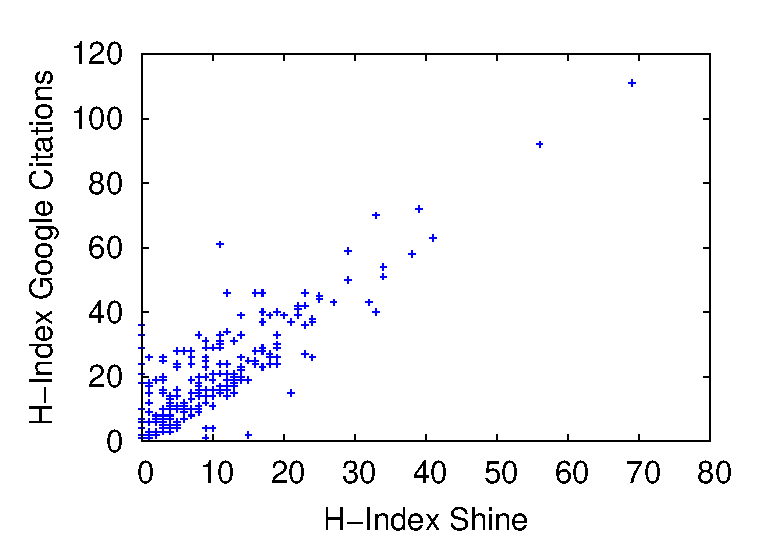
\includegraphics[scale=.5]{graficos/hindex/hindex_scatter_plot.eps}
\caption{Correlation between the inferred h-index and Google Citations one}
\label{fig:hindex_scatter_plot}
\end{figure}


However, there is one important limitation with this strategy.  As SHINE does not track all the existent computer science conferences, researchers' h-index might be underestimated when computed
with this data. To investigate this issue, we compared the h-index of a set of researchers with a profile on Google Scholar with their estimated h-index based on the SHINE data. For this, we
randomly selected 10 researchers for each conference from Table~\ref{tab:sigs_conference_period} and extracted their h-indexes from their Google Scholar profiles.  In comparison
with the h-index we estimated from SHINE, the Google scholar values are, on average, 50\% higher. Figure~\ref{fig:hindex_scatter_plot} shows the scatter plot for the two h-index
measures. We can note that although SHINE h-index is smaller, the two measures are highly correlated. The pearson correlation coefficient is 0.85, which indicates that researchers
might have proportional h-index estimations in both systems. 

\subsection{Setting the Thresholds}
\label{sub:thresholds}


There are two important thresholds in our approach we need to define to determine the core of a scientific community.  The first is related to the time window in which the 
community core is computed. In other words, should we compute the community core at each year, at each two years, or for a larger time window? The second threshold is related to the
size of the community core. As we define the core of a community as the top researchers in terms of their core score during a certain time window, it is important to define the
threshold for choosing the top ones.

Our strategy to define these two thresholds consists of varying each of them and quantifying how they impact on the changes on the members of the community core. To measure these
changes, we compute the resemblance metric, as used in~\cite{Viswanath:2009}, which measures the fraction of members in the core at time $t_0$ that remains in the core at the
time $t_1$. For each community, we varied the window size from 1 to 5 years and the size of the community core from 10\% to 60\% of the entire community.

Intuitively, high resemblance variations indicate bad threshold choices and, thus, we should seek for values in which threshold changes cause slight changes on resemblance.
Figure~\ref{fig:averange_values_resemblance} shows the resemblance values as a function of the window size, providing different curves for the community core size.  We chose the
SIGMOD and CHI communities for this analysis. The rest of the communities are omitted due to lack of space, but the same observations hold for them. By visual inspection we would set the core
size as 10\% due to the proximity of the curves, and the window size as 2 or 3, as most of the communities showed a more stable resemblance after these values. To help us decide, we
computed the angular coefficient for the 10\% core size curves of each community and obtained the average angular coefficient for them.  Based on this value, we chose the window
size for our experiments as 3 years.

\begin{figure}[!htb]
  \begin{center}
    \subfigure[SIGMOD]{%
      \label{fig:sigmod_slide_window_top_list}
      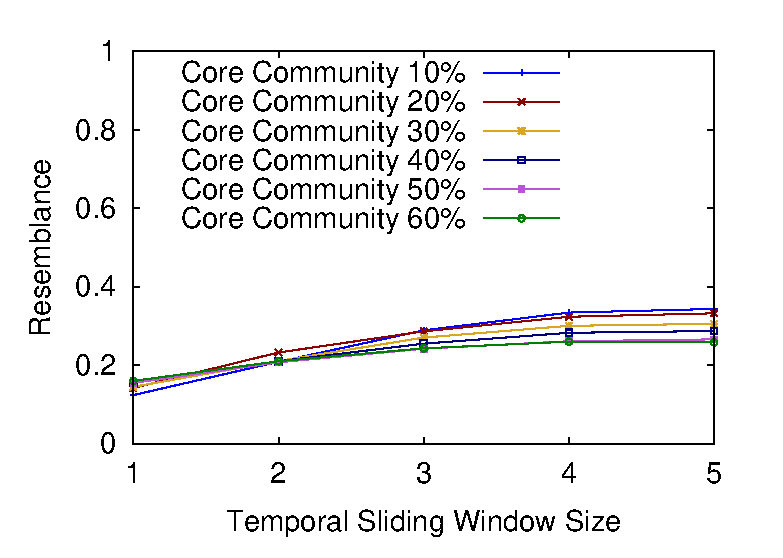
\includegraphics[scale=.33]{graficos/window_core_size/sigmod_slide_window_top_list.eps}
    }%
    \subfigure[CHI]{%
      \label{fig:chi_slide_window_top_list}
      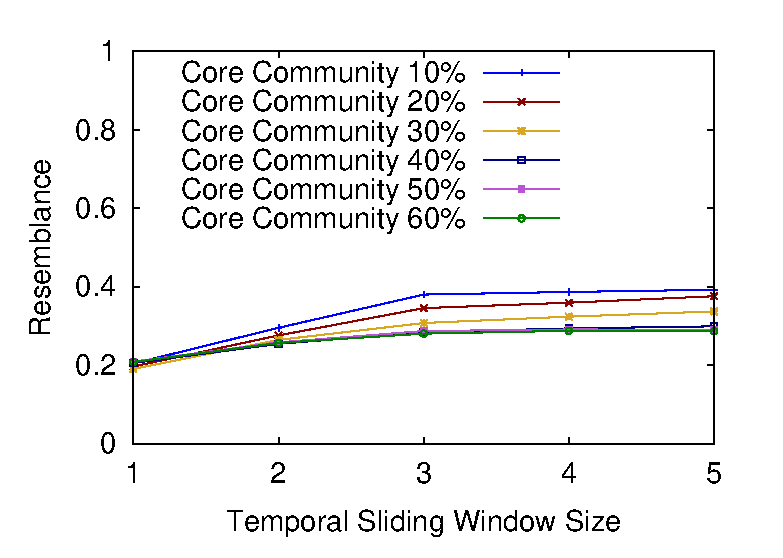
\includegraphics[scale=.33]{graficos/window_core_size/chi_slide_window_top_list.eps}
    }%
  \end{center}
\caption{Average of the values of resemblance}
 \label{fig:averange_values_resemblance}
\end{figure}


\subsection{Validation}

Based on the core score value, we expect that the members of the community core would be standing researchers that actively contribute with publications to a certain community.
The validation of this assumption is, by nature, subjective.  Thus, we provide next evidence that our approach correctly captures this expected characteristic.

First, we analyzed the core score of two WWW 2013 keynote speakers: Jon Kleinberg and Luis von Ahn.  Figure~\ref{fig:rank_core_score_authors} shows the ranking position in terms of
percentage (e.g., position 5\% of that community) of these two researchers in the communities they have published. The botton line divides the members of the community core from the others.
We can note that Jon Kleinberg was a member of the community core of STOC, a theoretical conference, for years. More precisely, he was part of the STOC core for twelve years,
publishing seven STOC papers in a single period of three years. With Kleinberg's involvement on KDD, he became less active in STOC and left the core of that community for some time.
During this period, he published several KDD papers, while his STOC publications were drastically reduced.  When it comes to Luis von Ahn, we can note that he is more active in
the CHI community, a community in which he published six papers along his academic life. He reached the core of the CHI community along three consecutive time windows,
publishing four CHI papers in a single period.



\begin{figure}[!htb]
  \begin{center}
    \subfigure[Jon Kleinberg]{%
      \label{fig:cc_kleinberg}
      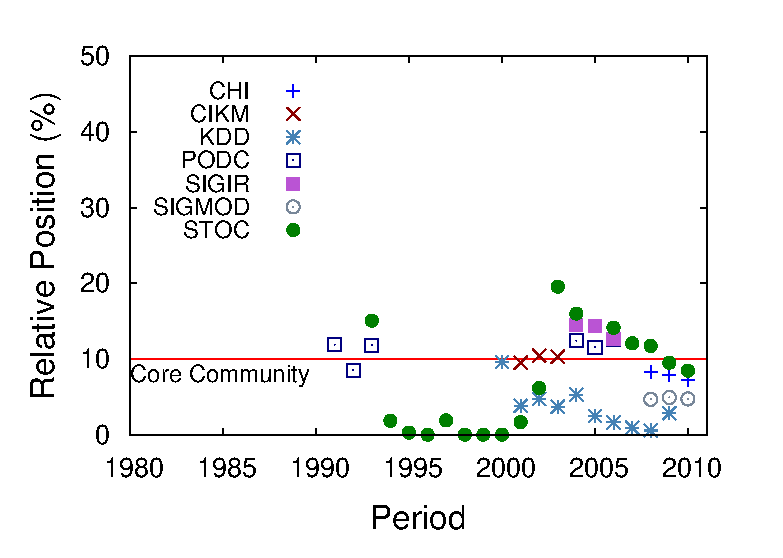
\includegraphics[scale=.33]{graficos/validacao_core_community/cc_kleinberg.eps}
    }%
    \subfigure[Luis von Ahn]{%
      \label{fig:cc_luis_von_ahn}
      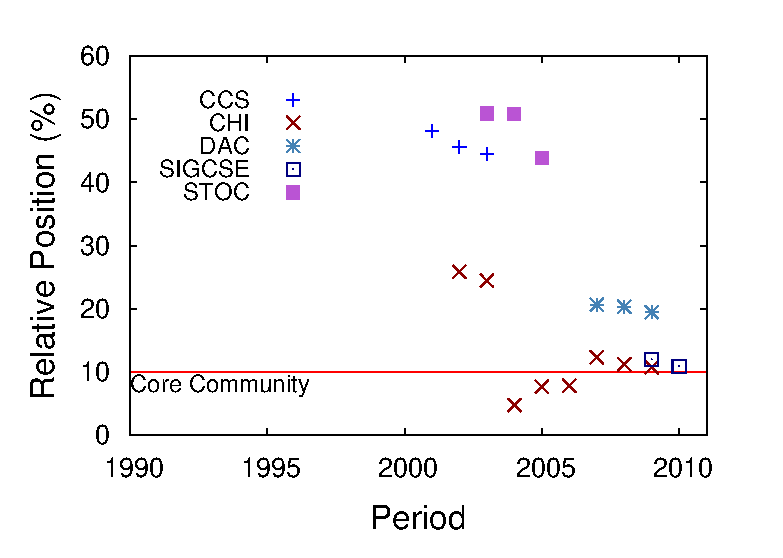
\includegraphics[scale=.33]{graficos/validacao_core_community/cc_luis_von_ahn.eps}
    }%
  \end{center}
\caption{Core score of two WWW 2013 keynote speakers}
 \label{fig:rank_core_score_authors}
\end{figure}


Next, we computed a ranking of researchers that appear most often in the community core of each scientific community. We chose the KDD, SIGCOMM, SIGIR, and SIGMOD communities to
show their top 20 researchers in Table~\ref{tab:authors_frequency_core_community}.  As we can note, several big names appear in this top list, including past keynote speakers of
these conferences as well as awarded researchers by their life time contributions in that community. Indeed, by analyzing the awarded researchers from each community we found that
a large fraction of them appeared in the community core at least one time in the conference history. More specifically, these fractions are 75\% of the awarded
KDD\footnote{http://www.sigkdd.org/awards\_innovation.php} members, 35\% for SIGCOMM\footnote{http://www.sigcomm.org/awards/sigcomm-awards}, 60\% for
SIGIR\footnote{http://www.sigir.org/awards/awards.html}, and 80\% for SIGMOD\footnote{http://www.sigmod.org/sigmod-awards}.  Except for SIGCOMM, a community with many sponsored
event that were not considered in our datasets, the other three communities presented very high numbers of awarded members that appear at least one time a community core. These
observations provide evidence that our approach correctly captures the notion of a scientific community core.


\begin{table*}[!htb]
\centering
\caption{Researchers who appear most often in the community core over the years}
\label{tab:authors_frequency_core_community}
{\small
\begin{tabular}{|c|c|c|c|} \hline
\bf{KDD} & \bf{SIGCOMM} & \bf{SIGIR} & \bf{SIGMOD}\\ \hline
Heikki Mannila$^\star$ & Scott Shenker$^\star$ & W. Bruce Croft$^\star$ & David J. DeWitt$^\star$\\ \hline
Jiawei Han$^\star$ & George Varghese & Clement T. Yu & Michael Stonebraker$^\star$\\ \hline
Eamonn J. Keogh & Hui Zhang & Susan T. Dumais$^\star$ & H. V. Jagadish\\ \hline
Martin Ester & Donald F. Towsley$^\star$ & James Allan & Rakesh Agrawal$^\star$\\ \hline
Bing Liu & Hari Balakrishnan & Justin Zobel & Christos Faloutsos\\ \hline
Padhraic Smyth$^\star$ & Ion Stoica & Alistair Moffat & Raghu Ramakrishnan\\ \hline
Charu C. Aggarwal & Srinivasan Seshan & Norbert Fuhr$^\star$ & Jiawei Han\\ \hline
Philip S. Yu & Deborah Estrin & James P. Callan & Gerhard Weikum\\ \hline
Ke Wang & David Wetherall & Yiming Yang & Philip A. Bernstein$^\star$\\ \hline
Hans-Peter Kriegel & Thomas E. Anderson & Edward A. Fox & Jeffrey F. Naughton\\ \hline
Rakesh Agrawal$^\star$ & Jennifer Rexford & Gerard Salton$^\star$ & Hector Garcia-Molina$^\star$\\ \hline
Jian Pei & Jia Wang & Ricardo A. Baeza-Yates & Michael J. Carey$^\star$\\ \hline
Wynne Hsu & Ratul Mahajan & Jian-Yun Nie & Joseph M. Hellerstein\\ \hline
Qiang Yang & Vern Paxson$^\star$ & Mark Sanderson & Philip S. Yu\\ \hline
Christos Faloutsos$^\star$ & Mark Handley & Charles L. A. Clarke & Divesh Srivastava\\ \hline
Huan Liu & Yin Zhang & Chris Buckley & Michael J. Franklin\\ \hline
Mohammed Javeed Zaki & Peter Steenkiste & Chengxiang Zhai & Jennifer Widom$^\star$\\ \hline
Pedro Domingos & Walter Willinger & Alan F. Smeaton & Hans-Peter Kriegel\\ \hline
Jon M. Kleinberg & Ramesh Govindan & Zheng Chen & Hamid Pirahesh\\ \hline
Vipin Kumar$^\star$ & Jon Crowcroft$^\star$ & Ophir Frieder & Surajit Chaudhuri$^\star$\\ \hline
\end{tabular}
\par\medskip\footnotesize{$^\star$ Researchers awarded by a lifetime of innovation and leadership inside that community.}
%\begin{tabular}{|c|l|l|l|l|} \hline
% & \bf{KDD} & \bf{SIGCOMM} & \bf{SIGIR} & \bf{SIGMOD}\\ \hline
%1\textsuperscript{st} & Heikki Mannila$^\star$ & Scott Shenker$^\star$ & W. Bruce Croft$^\star$ & David J. DeWitt$^\star$\\ \hline
%2\textsuperscript{nd} & Jiawei Han$^\star$ & George Varghese & Clement T. Yu & Michael Stonebraker$^\star$\\ \hline
%3\textsuperscript{rd} & Eamonn J. Keogh & Hui Zhang & Susan T. Dumais$^\star$ & H. V. Jagadish\\ \hline
%4\textsuperscript{th} & Martin Ester & Donald F. Towsley$^\star$ & James Allan & Rakesh Agrawal$^\star$\\ \hline
%5\textsuperscript{th} & Bing Liu & Hari Balakrishnan & Justin Zobel & Christos Faloutsos\\ \hline
%6\textsuperscript{th} & Padhraic Smyth$^\star$ & Ion Stoica & Alistair Moffat & Raghu Ramakrishnan\\ \hline
%7\textsuperscript{th} & Charu C. Aggarwal & Srinivasan Seshan & Norbert Fuhr$^\star$ & Jiawei Han\\ \hline
%8\textsuperscript{th} & Philip S. Yu & Deborah Estrin & James P. Callan & Gerhard Weikum\\ \hline
%9\textsuperscript{th} & Ke Wang & David Wetherall & Yiming Yang & Philip A. Bernstein$^\star$\\ \hline
%10\textsuperscript{th} & Hans-Peter Kriegel & Thomas E. Anderson & Edward A. Fox & Jeffrey F. Naughton\\ \hline
%11\textsuperscript{th} & Rakesh Agrawal$^\star$ & Jennifer Rexford & Gerard Salton$^\star$ & Hector Garcia-Molina$^\star$\\ \hline
%12\textsuperscript{th} & Jian Pei & Jia Wang & Ricardo A. Baeza-Yates & Michael J. Carey$^\star$\\ \hline
%13\textsuperscript{th} & Wynne Hsu & Ratul Mahajan & Jian-Yun Nie & Joseph M. Hellerstein\\ \hline
%14\textsuperscript{th} & Qiang Yang & Vern Paxson$^\star$ & Mark Sanderson & Philip S. Yu\\ \hline
%15\textsuperscript{th} & Christos Faloutsos$^\star$ & Mark Handley & Charles L. A. Clarke & Divesh Srivastava\\ \hline
%16\textsuperscript{th} & Huan Liu & Yin Zhang & Chris Buckley & Michael J. Franklin\\ \hline
%17\textsuperscript{th} & Mohammed Javeed Zaki & Peter Steenkiste & Chengxiang Zhai & Jennifer Widom$^\star$\\ \hline
%18\textsuperscript{th} & Pedro Domingos & Walter Willinger & Alan F. Smeaton & Hans-Peter Kriegel\\ \hline
%19\textsuperscript{th} & Jon M. Kleinberg & Ramesh Govindan & Zheng Chen & Hamid Pirahesh\\ \hline
%20\textsuperscript{th} & Vipin Kumar$^\star$ & Jon Crowcroft$^\star$ & Ophir Frieder & Surajit Chaudhuri$^\star$\\ \hline
%\end{tabular}
}
% \par\medskip\footnotesize{$^\star$ Researchers awarded by a lifetime of innovation and leadership inside that community.}
\end{table*}
% \let\thefootnote\relax\footnote{$^\star$ Researchers awarded by a lifetime of innovation and leadership inside that community.}
%  & \bf CIKM & \bf KDD &\bf  SIGIR & \bf SIGMOD\\ \hline
% 1\textsuperscript{st} & Philip S. Yu & Heikki Mannila & W. Bruce Croft* & David J. DeWitt*\\ \hline
% 2\textsuperscript{nd} & Jiawei Han & Jiawei Han & Clement T. Yu & Michael Stonebraker*\\ \hline
% 3\textsuperscript{rd} & Ling Liu & Eamonn J. Keogh & Susan T. Dumais* & H. V. Jagadish\\ \hline
% 4\textsuperscript{th} & Clement T. Yu & Martin Ester & James Allan & Rakesh Agrawal*\\ \hline
% 5\textsuperscript{th} & Christos Faloutsos & Bing Liu & Justin Zobel & Christos Faloutsos\\ \hline
% 6\textsuperscript{th} & James Allan & Padhraic Smyth & Alistair Moffat & Raghu Ramakrishnan\\ \hline
% 7\textsuperscript{th} & Elke A. Rundensteiner & Charu C. Aggarwal & Norbert Fuhr* & Jiawei Han\\ \hline
% 8\textsuperscript{th} & Ke Wang & Philip S. Yu & James P. Callan & Gerhard Weikum\\ \hline
% 9\textsuperscript{th} & Amr El Abbadi & Ke Wang & Yiming Yang & Philip A. Bernstein*\\ \hline
% 10\textsuperscript{th} & W. Bruce Croft & Hans-Peter Kriegel & Edward A. Fox & Jeffrey F. Naughton\\ \hline
% 11\textsuperscript{th} & Ming-Syan Chen & Rakesh Agrawal & Gerard Salton* & Hector Garcia-Molina*\\ \hline
% 12\textsuperscript{th} & Divyakant Agrawal & Jian Pei & Ricardo A. Baeza-Yates & Michael J. Carey*\\ \hline
% 13\textsuperscript{th} & C. Lee Giles & Wynne Hsu & Jian-Yun Nie & Joseph M. Hellerstein\\ \hline
% 14\textsuperscript{th} & Weiyi Meng & Qiang Yang & Mark Sanderson & Philip S. Yu\\ \hline
% 15\textsuperscript{th} & Berthier A. Ribeiro-Neto & Christos Faloutsos & Charles L. A. Clarke & Divesh Srivastava\\ \hline
% 16\textsuperscript{th} & M. Tamer \"Ozsu & Huan Liu & Chris Buckley & Michael J. Franklin\\ \hline
% 17\textsuperscript{th} & ChengXiang Zhai & Mohammed Javeed Zaki & ChengXiang Zhai & Jennifer Widom*\\ \hline
% 18\textsuperscript{th} & Javed A. Aslam & Pedro Domingos & Alan F. Smeaton & Hans-Peter Kriegel\\ \hline
% 19\textsuperscript{th} & Hans-Peter Kriegel & Jon M. Kleinberg & Zheng Chen & Hamid Pirahesh\\ \hline
% 20\textsuperscript{th} & Bing Liu & Vipin Kumar & Ophir Frieder & Surajit Chaudhuri*\\ \hline
